\documentclass[tikz]{standalone}

%: === FONT === (((
\usepackage{amssymb}
\usepackage{fontspec}
\setmainfont[
  BoldFont       = bodonibi,
	ItalicFont     = Century modern italic2.ttf,
	BoldItalicFont = bodonibi,
	SmallCapsFont  = lmromancaps10-regular.otf
]{Century_modern.ttf}
\DeclareSymbolFont{italics}{\encodingdefault}{\rmdefault}{m}{it}
\DeclareSymbolFontAlphabet{\mathit}{italics}
\ExplSyntaxOn
\int_step_inline:nnnn { `A } { 1 } { `Z }
 {  \exp_args:Nf \DeclareMathSymbol{\char_generate:nn{#1}{11}}{\mathalpha}{italics}{#1} }
\int_step_inline:nnnn { `a } { 1 } { `z } {  \exp_args:Nf \DeclareMathSymbol{\char_generate:nn{#1}{11}}{\mathalpha}{italics}{#1}}
\ExplSyntaxOff
% )))

\begin{document}

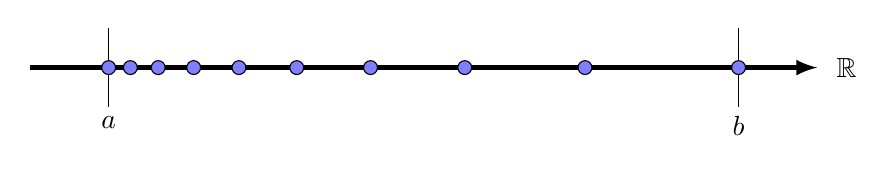
\begin{tikzpicture}[>=latex]

	\draw [ultra thick,->] (0,0) -- (10,0) node [right=1mm] {\(\mathbb{R}\)};
	\draw (1,0.5) -- (1,-0.5) node [below] {\(a\)};
	\draw (9,0.5) -- (9,-0.5) node [below] {\(b\)};
	\def\N{9}
	\foreach \n in {0,...,\N} 
	\filldraw [fill = white!50!blue, draw = black] 
	({pow(9,\n/\N)},0) circle (2.5pt);

\end{tikzpicture}

\end{document}
